\documentclass[tikz,border=8pt]{standalone}
\usepackage{tikz}
\usepackage{tkz-euclide}
\usepackage{amsmath, amssymb}

\usetikzlibrary{angles, quotes}

\begin{document}

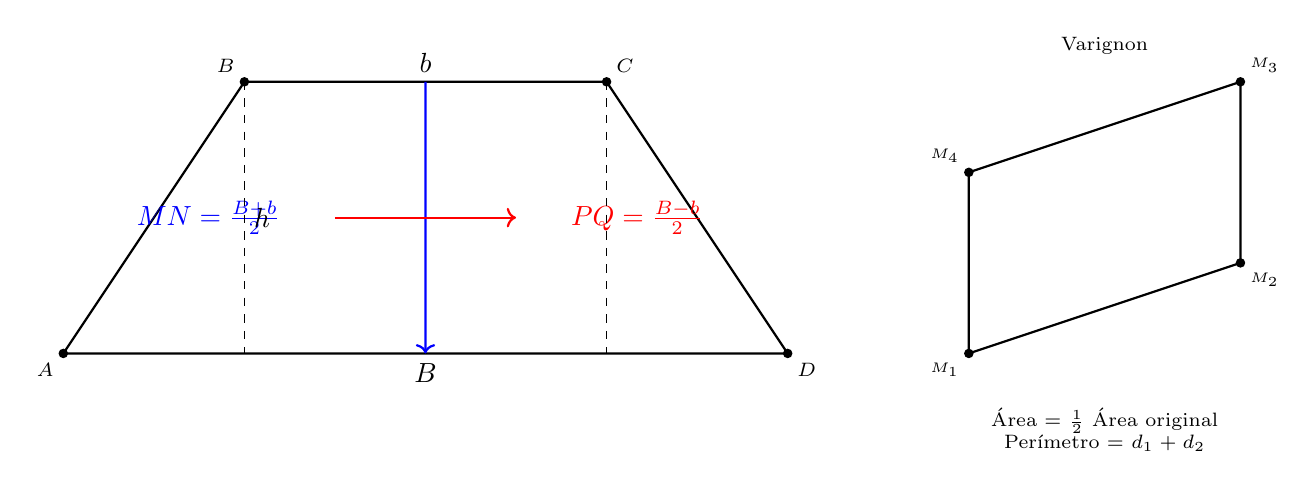
\begin{tikzpicture}[scale=1.15]

  % ---- Trapecio ABCD (B mayor abajo, b menor arriba) ----
  \coordinate (A) at (0,0);
  \coordinate (D) at (8,0);
  \coordinate (B) at (2,3);
  \coordinate (C) at (6,3);

  \draw[thick] (A) -- (B) -- (C) -- (D) -- cycle;

  % ---- Bases ----
  \node[below] at (4,0) {$B$};
  \node[above] at (4,3) {$b$};

  % ---- Puntos medios de lados laterales (mediana/base media) ----
  \coordinate (M_AD) at ($(A)!0.5!(D)$);
  \coordinate (M_BC) at ($(B)!0.5!(C)$);
  \draw[blue, thick, ->] (M_BC) -- (M_AD);
  \node[blue, left] at (2.5,1.5) {$MN = \frac{B+b}{2}$};

  % ---- Puntos medios de diagonales ----
  \coordinate (P_AC) at ($(A)!0.5!(C)$);
  \coordinate (Q_BD) at ($(B)!0.5!(D)$);
  \draw[red, thick, ->] (P_AC) -- (Q_BD);
  \node[red, right] at (5.5,1.5) {$PQ = \frac{B-b}{2}$};

  % ---- Altura ----
  \draw[dashed] (2,3) -- (2,0);
  \draw[dashed] (6,3) -- (6,0);
  \node[right] at (2,1.5) {$h$};

  % ---- Vértices ----
  \fill (A) circle (1.5pt) node[below left] {\scriptsize $A$};
  \fill (B) circle (1.5pt) node[above left] {\scriptsize $B$};
  \fill (C) circle (1.5pt) node[above right] {\scriptsize $C$};
  \fill (D) circle (1.5pt) node[below right] {\scriptsize $D$};

  % ---- Paralelogramo de Varignon (inset a la derecha) ----
  \begin{scope}[shift={(10,0)}]
    \coordinate (V1) at (0,0);
    \coordinate (V2) at (3,1);
    \coordinate (V3) at (3,3);
    \coordinate (V4) at (0,2);
    \draw[thick] (V1) -- (V2) -- (V3) -- (V4) -- cycle;
    \fill (V1) circle (1.5pt) node[below left] {\tiny $M_1$};
    \fill (V2) circle (1.5pt) node[below right] {\tiny $M_2$};
    \fill (V3) circle (1.5pt) node[above right] {\tiny $M_3$};
    \fill (V4) circle (1.5pt) node[above left] {\tiny $M_4$};
    \node[above] at (1.5,3.2) {\scriptsize Varignon};
    \node[below, align=center, text width=3cm, font=\scriptsize] at (1.5,-0.5) {
      Área = $\frac{1}{2}$ Área original\\
      Perímetro = $d_1 + d_2$
    };
  \end{scope}

\end{tikzpicture}

\end{document}
